\section{Introduction}
In Astronomy, instruments with higher angular resolution allows us to measure ever smaller structures in the sky. For Radio frequencies, the angular resolution is bound to the antenna dish diameter, which puts practical and financial limitations on the highest possible angular resolution. Radio Interferometers get around this limitation by using several smaller antennas instead. Together, they act as a single large antenna with higher angular resolution at lower financial costs compared to single dish instruments.

However, Radio Interferometers do not measure the pixels of the sky image. Instead, Radio Interferometers measure an incomplete set of Fourier components. The sky image has to be reconstructed from the measurements. This forms an ill-posed inverse problem: There are potentially many different images that fit the measurements, and 
from the measurements alone we cannot decide which image was actually observed.

Algorithms that solve the ill-posed Image Reconstruction problem. Find most likely images. Extensive Research in the last decades.

SKA wants to create Radio Interferometers on a new scale.
MeerKAT is the precursor of SKA-Mid. Create a new scale of Fourier measurements.
Push towards distributing
The Image Reconstruction Problem has to be solved with distributed computing.

Algorithms were developed before the advent of distributed computing. 
Distribution so far has been difficult. Only small number of nodes.


Target to distribute the image reconstruction
First tests


\subsection{Radio Interferometry System}\label{intro:sys}
This project is focused on distributing Image Reconstruction for Radio Interferometers, which is only one of three steps in the pipeline from measurements to the final image. We give a quick overview over the whole pipeline in figure \ref{intro:system} and how Radio Interferometers work in principle: The antennas observe the arriving electromagnetic wave, gets processed in three steps, Correlation, Calibration and Image Reconstruction. 

\begin{figure}[h]
	\centering
	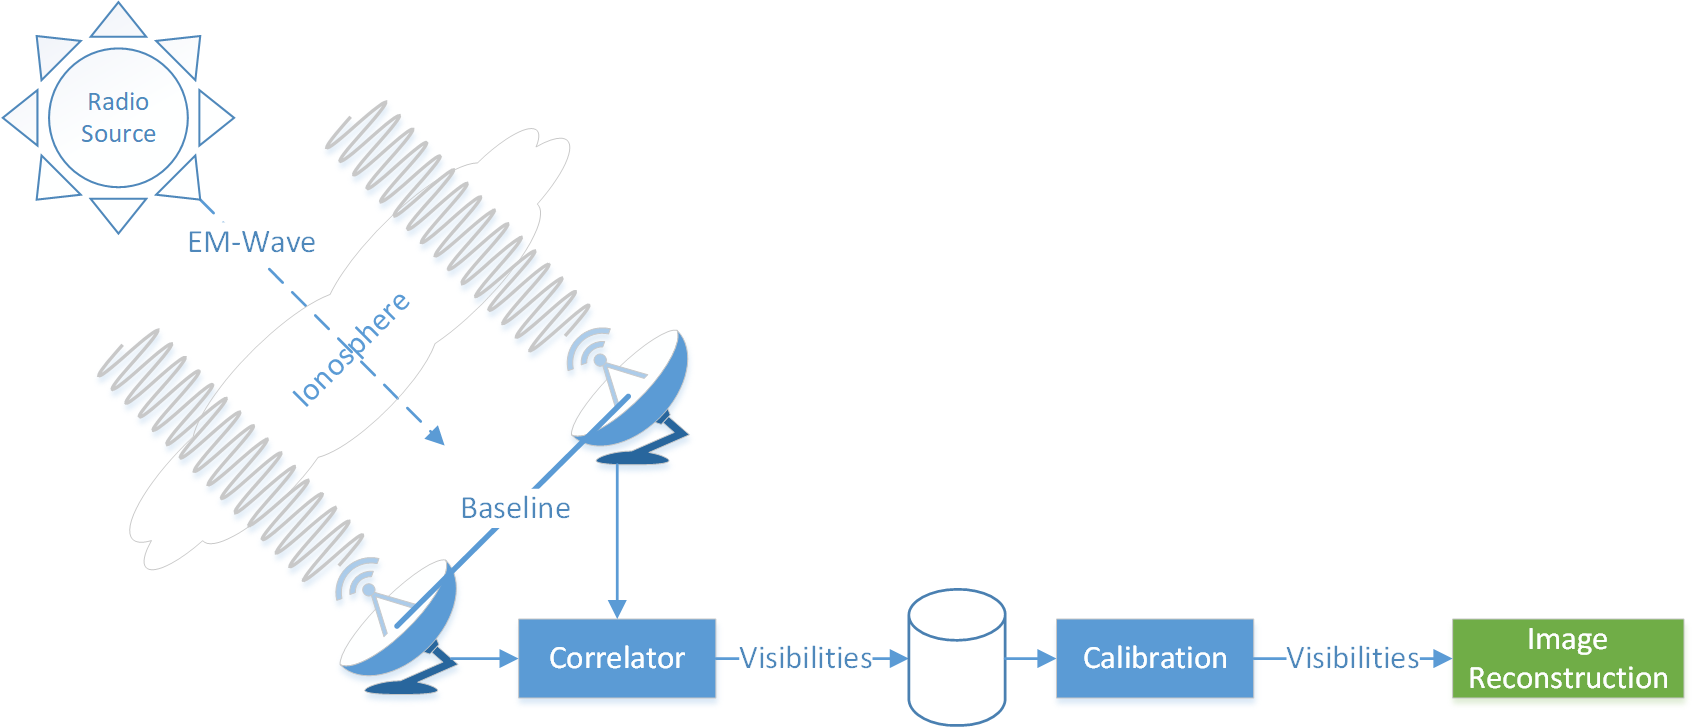
\includegraphics[width=0.80\linewidth]{./chapters/01.intro/system.png}
	\caption{Radio Interferometer System}
	\label{intro:system}
\end{figure}

First, the electromagnetic wave gets measured by the different antennas of the interferometer. The measurements of each antenna pair get correlated into a complex-valued Fourier Component (called Visibility in Radio Astronomy). Each antenna pair measures a noisy amplitude and phase of a single Visibility (Fourier Component) of the sky image. The distance and orientation of the antenna pair relative to the incoming signal, called the baseline, dictates which Visibility gets measured. The longer the baseline the higher-order Visibility gets measured, resulting in a higher angular resolution. After correlation, the Visibility data is saved for later processing.

The Calibration step is done after all Visibility data has been recorded. This step corrects the amplitude and phase of the measurements for varying antenna sensitivities, pointing errors and other effects. Also, this step removes corrupted data from the measurements. After the Visibilities are calibrated, we can average the measurements and reduce the data volume by several factors. Typically, averaging is done to reduce the runtime costs of the Image Reconstruction step.

The Image Reconstruction step takes the calibrated, and potentially averaged down Visibility data and finds the most likely observed image of the sky. Although the Interferometer produces a potentially large number of Visibilities, they are incomplete: For example an Interferometer with dish-antennas is typically blind to the microwave background radiation. The largest structures in the image it can detect depends on the shortest baseline. Since the antennas have to be at least the dish-diameter placed apart, the Interferometer is simply blind to very large structures in the sky image, like the microwave background radiation. This property makes Image Reconstruction Problem ill-posed. In the Image Reconstruction step, we therefore have to find the most likely image which fits the measurements.

\subsubsection{Earth's rotation and arbitrary large Number of Visibilities}
To improve the final image, we want to measure as many different Visibilities as possible. Modern Radio Interferometers use the the earth's rotation to change the baselines. When the earth rotates, it modifies the length of the baseline and by extent, what Visibilities get measured. Modern Interferometer can produce an almost arbitrary large number of measurements by just increasing the observation time.

The data volume can be averaged down in the Calibration step. However, with self-calibration, the Image Reconstruction is tasked with solving both the most likely image and the calibration parameters at the same time. This further improves the reconstruction quality\cite{Wiauxselfcal}, but requires the Image Reconstruction step to handle all the Visibility data.

Modern Radio Interferometers can produce an almost arbitrary large number of measurements. The reconstruction quality benefits from a large number of different Visibility measurements. The two main limiting factors however, are the cost of data storage and the scalability of the Image Reconstruction algorithm.


\subsection{The Image Reconstruction Problem}\label{intro:reconstruction}
For Radio Interferometers, Image Reconstruction forms an ill-posed inverse problem. There are potentially many different images that fit the measurements. The Image Reconstruction is tasked with finding the most likely image $I()$ given the (calibrated) Visibility measurements $V()$.  Figure \ref{intro:inversefig} shows an example from a MeerKAT observation for $V()$ and $I()$. The image \ref{intro:inversefig:uvspace} shows the incomplete sampling in the Fourier space. The sample density decreases away from the center\footnote{The center has actually no samples, since the MeerKAT Radio Interferometer uses antenna's with dishes. Due to the resolution, it might not be visible in the image \ref{intro:inversefig:uvspace}.}. The observed image \ref{intro:inversefig:reconstruction} contains two classes of structure, point sources and extended emissions. Point sources arise from stars and other distant objects, their emissions are concentrated around a single pixel. Extended emissions arise from hydrogen clouds and other sources which span an area of several arc-seconds of the sky. Or more formally, we want to invert the measurement equation \eqref{intro:inverseproblem} of the radio interferometer and retrieve the observed image $I()$. As we will see, this is an ill-posed inverse problem, and we have a large number of images that fit the measurements.

\begin{figure}[htp]
	% preliminary
	\sbox\twosubbox{%
		\resizebox{\dimexpr.9\textwidth-1em}{!}{%
			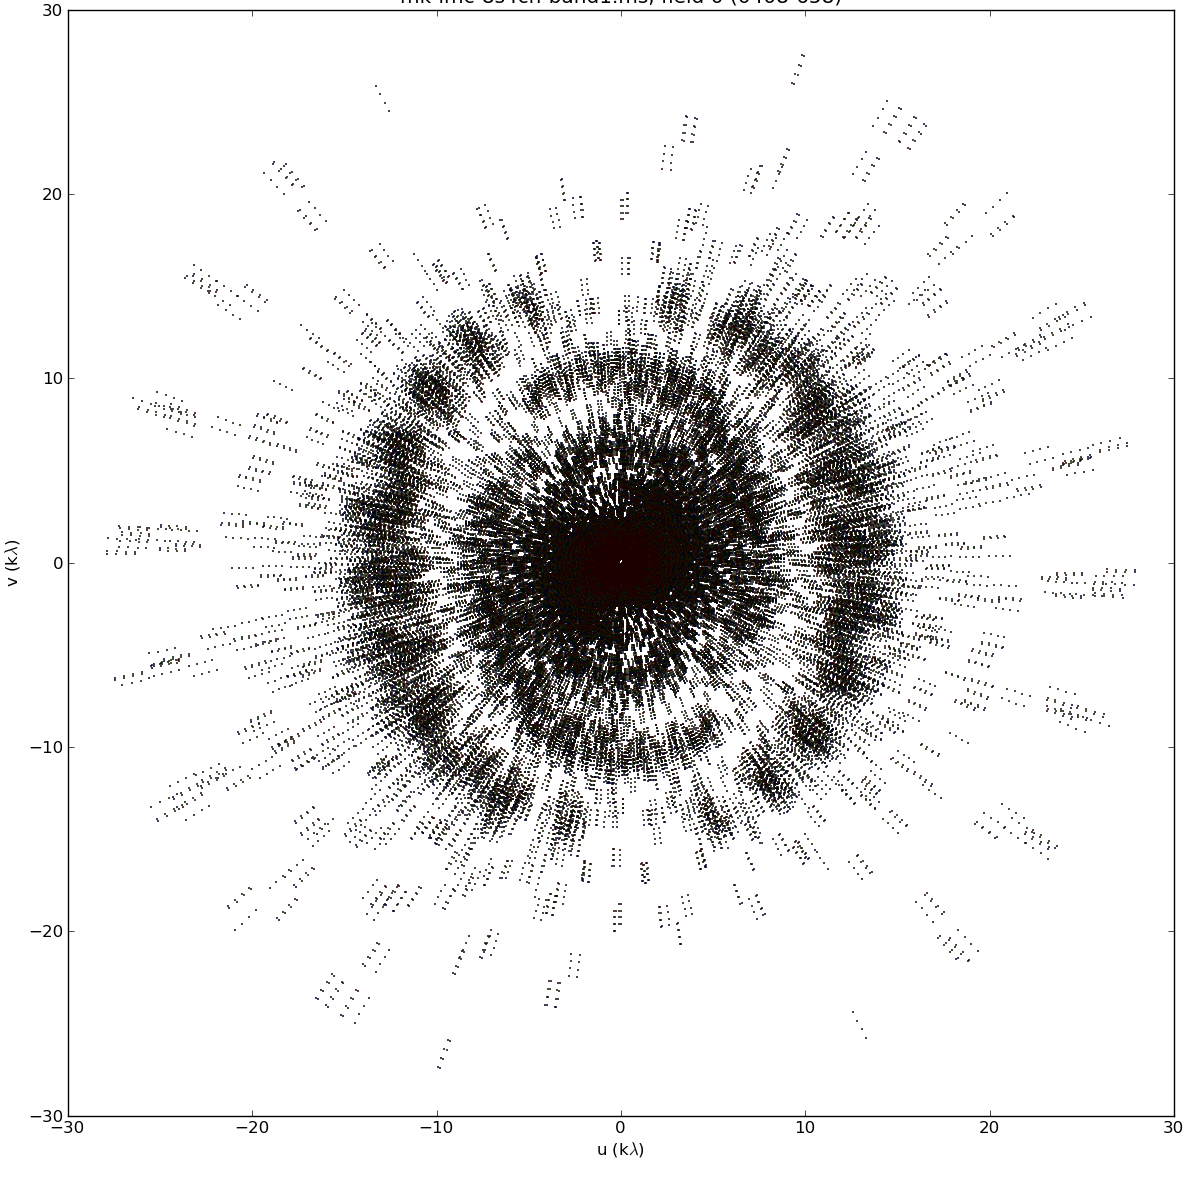
\includegraphics[height=3cm]{./chapters/01.intro/meerkat_uv2.png}%
			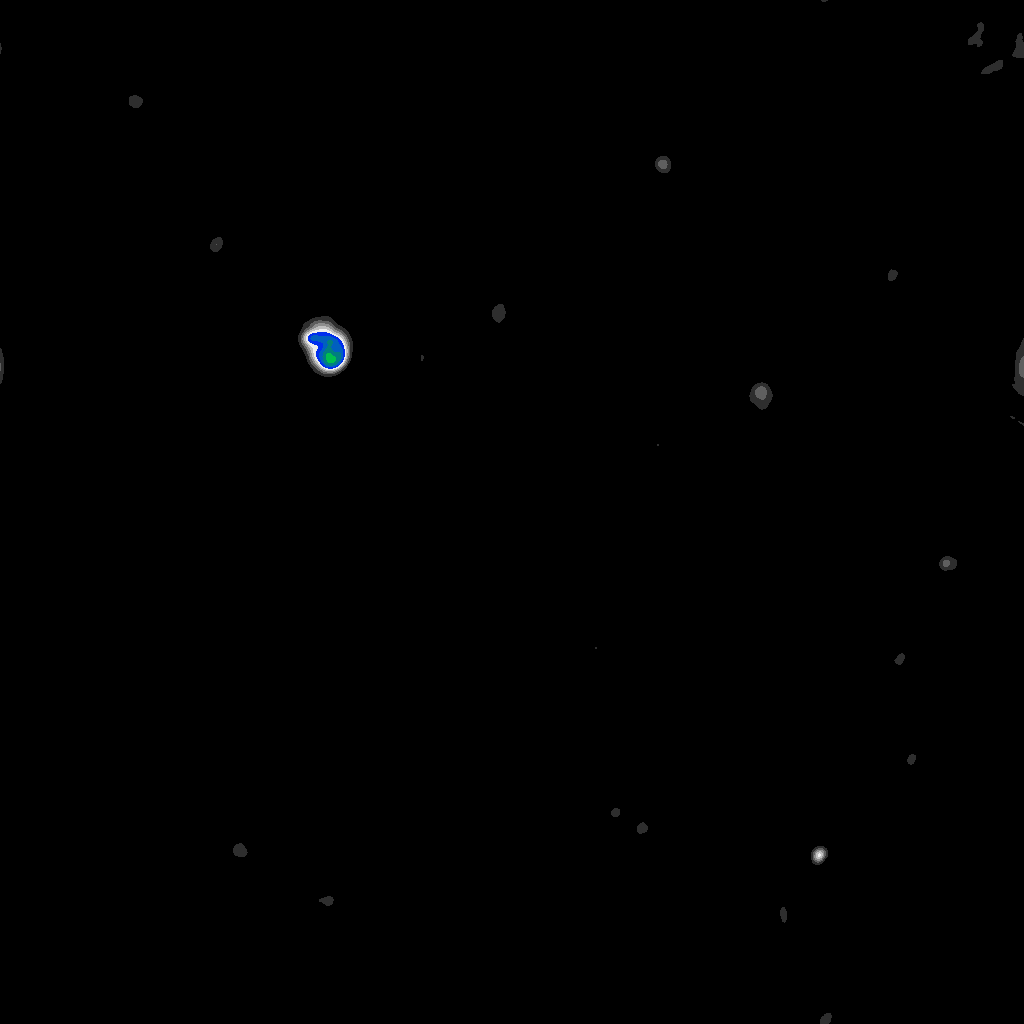
\includegraphics[height=3cm]{./chapters/01.intro/mk2/clean.png}%
		}%
	}
	\setlength{\twosubht}{\ht\twosubbox}
	
	% typeset
	\centering
	\subcaptionbox{Measurements $V()$ in the $uv$-plane.\label{intro:inversefig:uvspace}}{%
		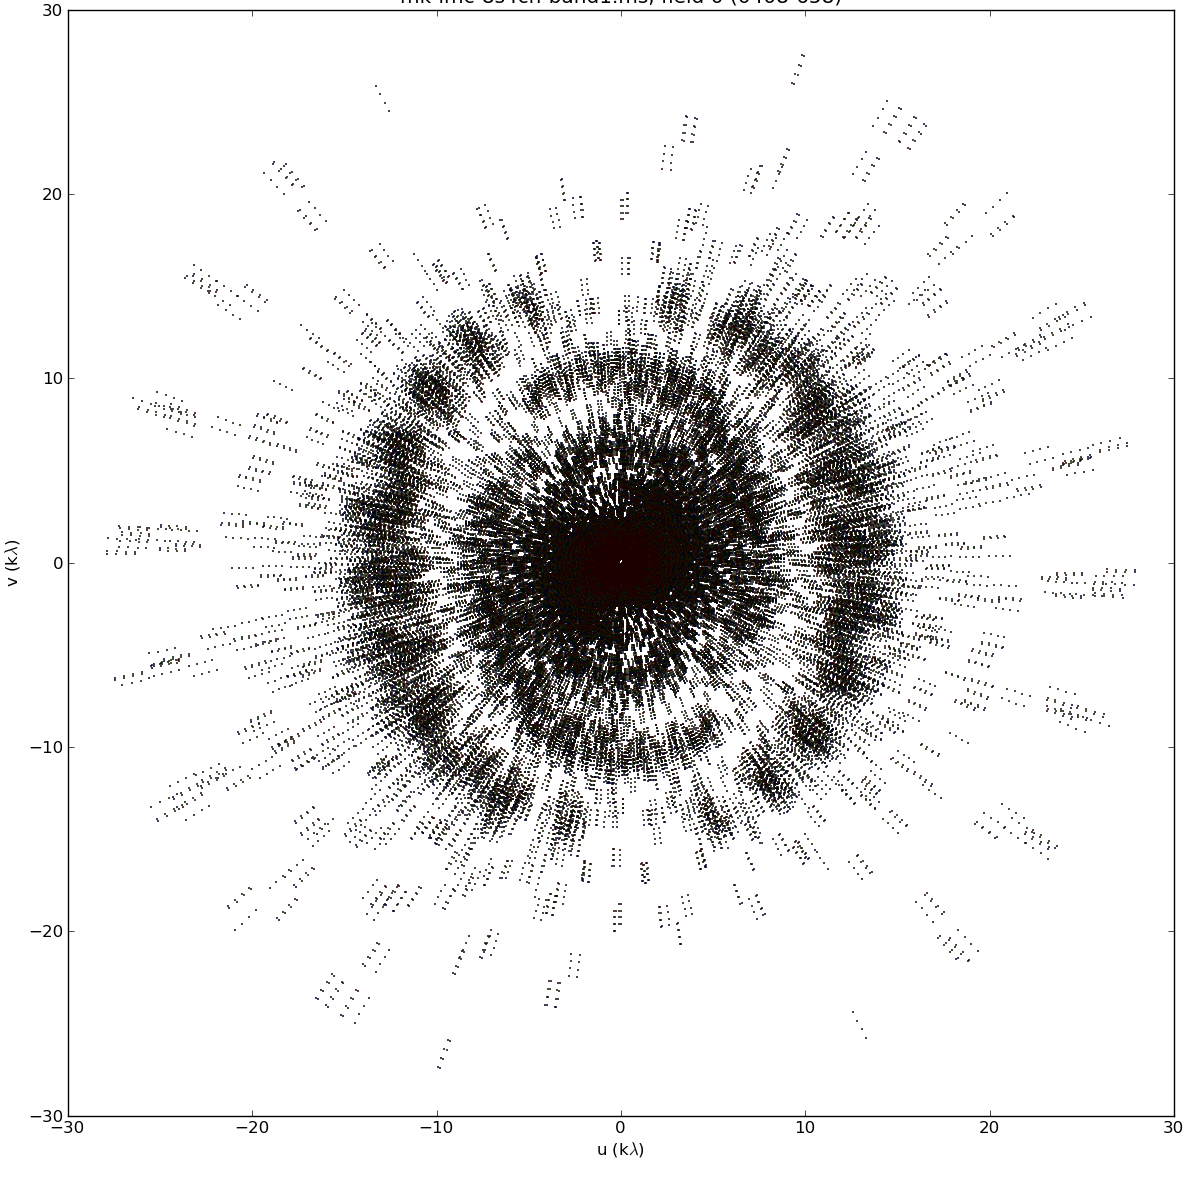
\includegraphics[height=\twosubht]{./chapters/01.intro/meerkat_uv2.png}%
	}\quad
	\subcaptionbox{The observed image $I()$.\label{intro:inversefig:reconstruction}}{%
		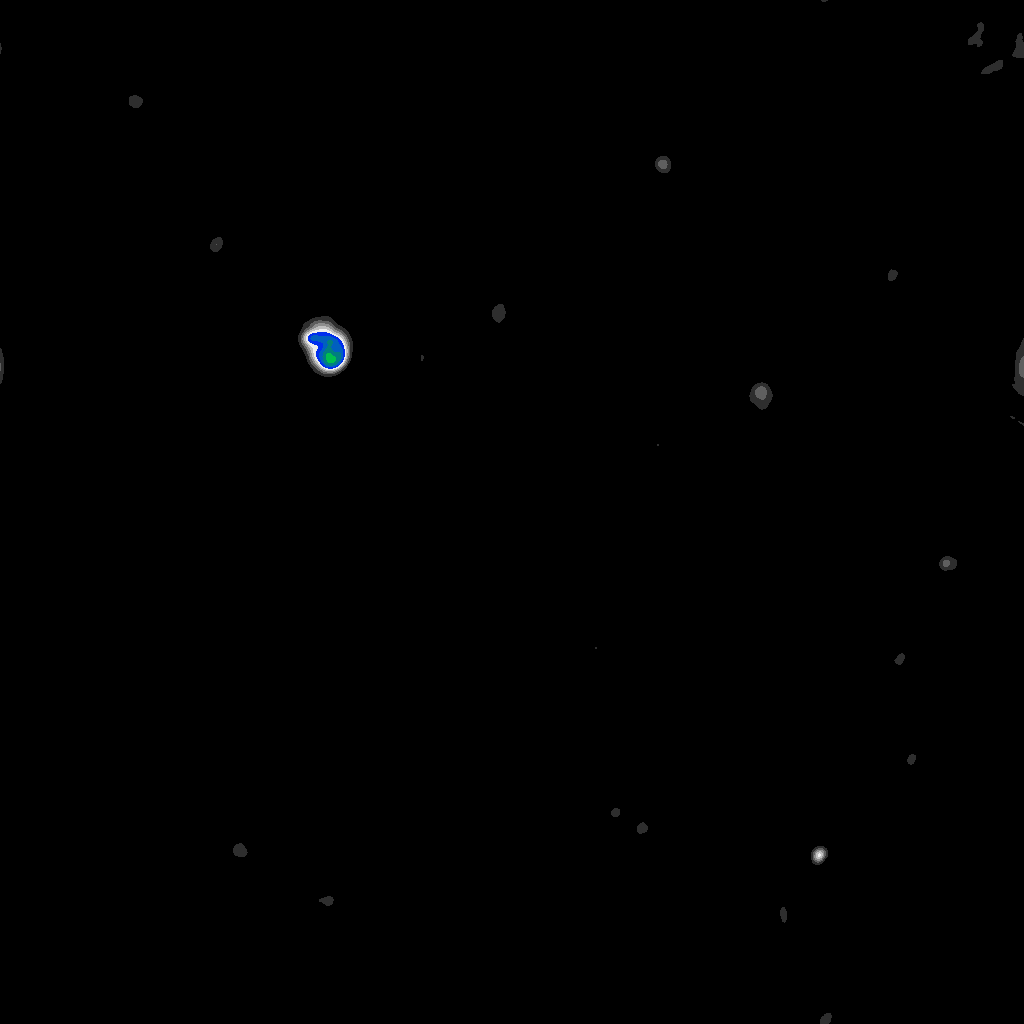
\includegraphics[height=\twosubht]{./chapters/01.intro/mk2/clean.png}%
	}
	\caption{The Image Reconstruction Problem}\label{intro:inversefig}
\end{figure}

Let us look at the measurement equation \eqref{intro:inverseproblem} in more detail. It consists of three parts: The Visibility measurements $V(u,v,w)$, the observed image with a normalization factor $\frac{I(x, y)}{c(x, y)}$ and the Fourier Transform $e^{2 \pi i [\ldots]}$. $u$ $v$ and $w$ represent the axes in the Fourier Domain, while the $x$ and $y$ axes represent the angles away from the image center. A pixel in $I(x,y)$ represents how much radio emission was measured from a the direction $x,y$.

\begin{equation}\label{intro:inverseproblem}
V(u, v, w) = \int\int  \frac{I(x, y)}{c(x, y)}  e^{2 \pi i [ux+vy+ w(c(x, y) - 1)]} \: dx \: dy \:,  \quad c(x,y) = \sqrt{1 - x^2 - y ^2}
\end{equation}

The radio interferometer essentially observes the sky in the Fourier domain. If we want to retrieve the observed sky image $I()$, all we need to do in theory is calculate the inverse Fourier Transform. However, the inverse Fourier Transform does not give us the observed image $I()$, because the measurements $V()$ are incomplete.

Note that the Visibilities $V(u,v,w)$ are three dimensional, while the image $I(x,y)$ only has two. However, also note that the third component $w$ only depends on the directions $x$ and $y$. In a sense, the Visibilities $V()$ and the Image $I()$ have a two dimensional Fourier relationship ($V(u,v,w) = \int\int I(x,y) e^{2 \pi i [ux+vy]} \: dx \: dy$), but with a directionally dependent correction factor $e^{2 \pi i [\ldots +w(c(x, y) - 1)]}$. 

The third component $w$ is an example of a Directionally Dependent Effect (DDE) which have a tendency to increase the runtime costs of the Image Reconstruction. The $w$-component keeps us from using the Fast Fourier Transform (FFT) for the measurement equation \eqref{intro:inverseproblem}. Research in this area tries to use approximations which lets us use faster algorithms like the FFT, and correct for DDE's accurately enough \cite{veenboer2017image, offringa2014wsclean, pratley2018fast}. In this project, the $w$-correction is the only DDE we handle.

%---------------------------------------------------------------------------------- Everything below this line needs to be reworked
\subsubsection{System of Linear Equations}\label{intro:linear}
Even though the Fourier Transform in equation \eqref{intro:inverseproblem} contains a $w$-correction factor, $V()$ and $I()$ have still a linear relationship. This means we can represent the Image Reconstruction Problem as a system of linear equations: \eqref{intro:linear:linear}. $F$ is the Fourier Transform with $w$-correction, $x$ is the image we are searching and $V$ are the measured Visibilities\footnote{$V$ in the equation \eqref{intro:linear:linear} is a vector. We use the lower-case $v$ to denote the axis in the Fourier space $uvw$, and the upper-case letter to denote the Visibility vector.}.

All the relevant deductions can be made in this.

\begin{equation}\label{intro:linear:linear}
\underset{x}{find}\quad V = Fx
\end{equation}

Under-Determined system, because $V$ is incomplete. We cannot get the observed image $x$
Add prior information. We know the image contains hydrogen clouds and distant stars. We can use this information and find the most likely image.

\begin{equation}\label{intro:linear:compressed}
\underset{x}{minimize} \: \left \| V - Fx \right \|_2^2 + \lambda P(x)
\end{equation}

This is a minimization problem, where we have the data term and regularization term. Data term forces image to be close to the measurements. Regularization term penalizes unlikely images. What are the chances of




As we discussed in section \ref{intro:sys}, Radio Interferometers can produce an almost arbitrary large number of Visibilities. In practice, we often reconstruct images with far fewer pixels than Visibility measurements, making the equation \eqref{intro:linear:linear} an over-determined problem. Meaning equation \eqref{intro:linear:linear} is either consistent and has a unique solution $x$, or is inconsistent with no solutions. Sadly, the Visibility measurements are subject to noise. The equation \eqref{intro:linear:linear} is inconsistent does not have a solution. To solve the Image Reconstruction Problem, we need to account for noise in the measurements, which leads us to a new inequality \eqref{intro:linear:l2}.

\begin{equation}\label{intro:linear:l2}
\underset{x}{find} \: \left \| V - Fx \right \|_2^2 < \epsilon
\end{equation}

We use the L2 norm and find the solution $x$ which, when the Fourier Transform is applied, has the smallest distance to the measurements $V$. The L2 norm leads to a strictly-convex function, meaning \eqref{intro:linear:l2} has only one minimum, and we can use convex optimization techniques to find it. So the question arises, is the observed image $I()$ located at the global minimum of \eqref{intro:linear:l2}? Although we have more measurements than pixels in the reconstruction, the set of Visibilities are still incomplete. They shift the observed image some distance away from the global minimum of \eqref{intro:linear:l2}. From the measurements alone, we cannot locate the observed image. We know it is near the global minimum, but we do not know where it is. The equation \eqref{intro:linear:l2} has many candidate solutions $x$, one of which is the observed image.  From the measurements alone, we cannot decide which candidate was the observed image, and \eqref{intro:linear:l2} is an ill-posed inverse problem. 

Intuitively, the incomplete measurements allow the pixels $x$ in the reconstruction to form physically implausible solutions. By including prior information, we can distinguish between likely and unlikely candidates of \eqref{intro:linear:l2}, and hopefully find the observed image. We can use the Theory of Compressed Sensing allows us to encode prior information about the image, and find the most likely solution to the ill-posed Image Reconstruction Problem.

\subsubsection{Theory of Compressed Sensing}
RIP of F

Recently, the Compressed Sensing sampling theorem has emerged\cite{candes2006robust, donoho2006compressed}, and has applications in data compression, de-noising\cite{zhu2009new}, and image reconstruction. For our intends and purposes, the Theory of Compressed Sensing gives us a way to encode prior information into the Image Reconstruction Problem. In essence, we choose a dictionary of basis functions $D$ to represent our image $x = D\alpha$. With the appropriate dictionary $D$, the most likely solution is the one with the fewest non-zero components in $\alpha$, and we arrive at the minimization objective \eqref{intro:linear:compressed:lasso} to solve our Image Reconstruction Problem. But first, let us look at how we chose the dictionary $D$ and how we include prior information in more detail.

We can always represent the image in a different space, for example with Haar-wavelets. In that case $D$ in $x = D\alpha$ is a dictionary of Haar-Wavelets, $\alpha$ is the Haar-Wavelet component vector and $x$ are the pixel values of our image. 
Natural images are sparse in Haar-Wavelet space. Few non-zero components in $\alpha$
If the natural image is corrupted with noise, it tends to affect all $\alpha$'s equally, meaning it is not sparse any more. However, the most significant components are still the original ones. So by searching for a solution which is sparse in Haar-Wavelet space, we can de-noise the image.

For our Image Reconstruction Problem, we need a dictionary $D$ in which our observed image can be sparsely represented.
If we choose the right $D$, the Theory of Compressed Sensing guarantees us the most likely image is the observed one.
We search for the image $x$ which is as close to the measurements as possible, but also has the fewest non-zero components $\alpha$. We can formulate this as a LASSO minimization problem \eqref{intro:linear:l2}.

\begin{equation}\label{intro:linear:compressed:lasso}
\underset{x}{minimize} \: \left \| V - Fx \right \|_2^2 + \lambda \left \| D^{-1}x \right \|_1 
\end{equation}

The objective contains two terms: The data term $\left \| V - Fx \right \|_2^2$, which is identical to the previous inequality \eqref{intro:linear:l2}, and the regularization term $\lambda \left \| D^{-1}x \right \|_1$, which enforces sparsity in our Dictionary.
Reconstruction quality depends on the choice of $D$
Radio Astronomy three different $D$ are in wide use, Starlets, Daubechies Wavelets, and sparsity in image domain.
Starlets and daubechies lead to better reconstruction quality, 

So we need a Regularization Dicitionary $D$, which captures the prior information we have about the image. Then, we can use convex optimization techniques to minimize the objective \eqref{intro:linear:compressed:lasso}.


\subsubsection{Different Representations for the LASSO Objective}\label{intro:linear:repr}
There are different ways to represent the LASSO objective \eqref{intro:linear:compressed:lasso}. Has the data term in the Fourier space, and reconstructs the image directly. We have different design decisions here. We can choose the Data term to be either in Fourier or image space, and we can set the Variables to be in either image, uniform Fourier or in the sparse space.

These possibilities arise from the Fourier Transform Matrix $F$, shown in equation \eqref{intro:linear:repr:fourier}. The first line shows the normal Fourier transform, from image $x$ into Visibilities $V$. Since $x$ is in a uniformly-sampled space, we can factorize $F$ into the FFT and the masking matrix $M$ and we arrive at the second line of equation \eqref{intro:linear:repr:fourier}. $M$ is essentially a matrix contains values between zero and one.
Represents the degradation due to incomplete measurements. 

\begin{equation} \label{intro:linear:repr:fourier}
\begin{split}
V &= Fx\\
V &= M\: FFT(x)\\
V &= M\: V_2\\
I_{Dirty} &= x \star PSF
\end{split}
\end{equation}

We can use the matrix $M$ directly, and use it to transform from uniformly sampled Visibilities $V_2$ to non-uniformly sampled Visibilities $V$, arriving at line three of equation \eqref{intro:linear:repr:fourier}.

Since a multiplication in Fourier space is a convolution in image space, we can also represent the masking matrix $M$ as a Point Spread Function $PSF$ in image space. Degradation is a convolution. $I_{Dirty}$ calculation is a Fourier Transform of the measurements. So we need to solve a deconvolution problem.
DIRTY IMAGE

All these lines are of \eqref{intro:linear:repr:fourier} all represent the Image Reconstruction Problem in different spaces. For example, if we change the data term in our LASSO objective from $\left \| V - Fx \right \|_2^2$ to a deconvolution $\left \| I_{Dirty} - x \star PSF \right \|_2^2$ we arrive at the same global minimum. But, in Radio Astronomy, the images are magnitudes smaller than the calibrated Visibility measurements $V$.
Reducing the problem size.
In practice, we have an accuracy issue with the $PSF$, since it is not constant. The $PSF$ changes over the image due to DDEs like $w$-correction.


\begin{equation} \label{intro:linear:repr:deconv}
\begin{split}
\underset{x}{minimize}\: \left \| V - Fx \right \|_2^2 + &\lambda \left \| D^{-1}x \right \|_1  \\
\underset{x}{minimize}\: \left \| I_{Dirty} - x \star PSF \right \|_2^2 + &\lambda \left \| D^{-1}x \right \|_1
\end{split}
\end{equation}

We will use deconvolution in the state-of-the-art.

Explain data space, reconstruction space and regularization space,

We can set the data term in our LASSO objective to either Visibility or image space. The reconstruction space has three possible design choices, which leads to three different LASSO objectives: Analysis, in-painting and synthesis.

\begin{alignat}{2}
\text{analysis:}\: \underset{x}{minimize}\:& \left \| V - Fx \right \|_2^2 + &\lambda \left \| D^{-1}x \right \|_1  \\
\text{in-painting:}\: \underset{V_2}{minimize}\:& \left \| V - MV_2 \right \|_2^2 + &\lambda \left \| D^{-1}F^{-1}V_2 \right \|_1 \label{intro:linear:repr:in} \\
\text{synthesis:}\: \underset{\alpha}{minimize}\:& \left \| V - FD\alpha \right \|_2^2 + &\lambda \left \| \alpha \right \|_1  
\end{alignat}

Analysis, standard formulation.

To our knowledge, in-painting \eqref{intro:linear:repr:in} is not used for the Image Reconstruction Problem. Difficulty in the Regularization term. 

Synthesis reconstructs in the sparse space, increases the number of free variables, we have at least as many $\alpha$ than $x$. But, we do not need the Matrix $D^{-1}$, which for certain spaces may not even be defined. We can use over-complete representations.
Why use over-complete? More freedom?


%^^^^^^^^^^^^^^^^^^^^^^^^^^^^^^^^^^^^^^^^^^^^^^^^^^^^^^^^^^^^^^^^^^^^^^^^^^^^^^^^^Everything ABOVE this line needs to be reworked


\subsection{Radio interferometric image reconstruction in practice}\label{intro:major}
We know how to solve the ill-posed image reconstruction problem in theory. We formulate a minimization problem \eqref{intro:linear:compressed}, specify a prior function that capture our prior knowledge, and find the optimum image with an appropriate optimization algorithm. In practice however we have a hard time representing the dense Fourier Transform matrix $F$ in the equation \eqref{intro:linear:compressed}. It is the size of number of visibilities times pixels in the reconstruction. Even older radio interferometers easily produce several million visibilities, with a million pixels in the reconstructed image. We cannot represent $F$ explicitly. However, we can reformulate the image reconstruction \eqref{intro:linear:compressed} as a deconvolution problem, which reduces the dimensions of the measurement $V$ and removes the large Fourier transform matrix $F$ from the minimization objective.

\subsubsection{Reformulating as a deconvolution problem}\label{intro:major:reformulation}
The Fourier transform matrix $F$ in \eqref{intro:linear:compressed} is a product of two operations: The Fourier transform $F$, and the masking operator $M$. The Fourier transform was established in section \ref{intro:reconstruction}. The masking operator is simply a matrix with zero entries for all Fourier components invisible to the instrument. So far, $M$ was implicitly contained in $F$ of \eqref{intro:linear:compressed}. To derive the deconvolution problem, we represent $M$ explicitly. For the sake of demonstration, let us assume our visibility measurements $V(u, v ,w)$ lie on a discrete grid. $V(u, v, w)$ is zero for all components that the interferometer could not measure. We then can represent the transformation from image to visibility space with the Fourier transform $F$ followed by a masking operation $M$, and we arrive at the image reconstruction problem \eqref{intro:major:reformulation:factor}. This is identical to \eqref{intro:linear:compressed}, except for the factorization of $F$.

\begin{alignat}{2}
\text{original:} \quad \underset{x}{minimize}\:& \left \| V - M Fx \right \|_2^2 + &\lambda P(x) \label{intro:major:reformulation:factor}\\ 
\text{in-painting:} \quad\underset{V_2}{minimize}\:& \left \| V - M V_2 \right \|_2^2 + &\lambda P(F^{-1}V_2) \label{intro:major:reformulation:fourier} \\
\text{deconvolution:} \quad \underset{x}{minimize}\:& \left \| I_{dirty} - x * PSF \right \|_2^2 + &\lambda P(x) \label{intro:major:reformulation:deconv}
\end{alignat}

Note that $M$ represents the degradation, the corruption introduced by incomplete sampling in the visibility space. $M$ is the important operator. The measurements $V$, or the reconstructed image $x$ can be in any space we wish. For example, we do not actually need to reconstruct the image in image space. In theory, we can reformulate an equivalent problem \eqref{intro:major:reformulation:fourier}, in which we in-paint the missing visibilities. Or, we can use the Fourier transform on the visibility measurements $V$ and the masking operator $M$, which leads us to the deconvolution problem \eqref{intro:major:reformulation:deconv}. 

Since the deconvolution formulation is vital for the major/minor cycle architecture, we have a closer look at \eqref{intro:major:reformulation:deconv}. The effect of incomplete sampling in Fourier space is equal to a convolution with a Point Spread Function $PSF$ in image space. I.e. $PSF = F^{-1}M$. The measurements are now represented as the "dirty" image, $I_{dirty} = F^{-1}V$. We try to find the deconvolved image $x$, while only knowing the convolution kernel $PSF$ and the convolved, dirty image $I_{dirty}$. This is still an ill-posed inverse problem. We have potentially many different deconvolutions that fit the dirty image, and we search the most likely candidate according to some prior $P(x)$. 

The deconvolution \eqref{intro:major:reformulation:deconv} and the original image reconstruction problem \eqref{intro:linear:compressed} are equivalent. Both arrive at the same result. But the deconvolution problem is easier to handle in practice: $I_{dirty}$ and $PSF$ are generally more compact representations of $V$ and $M$. There is one last issue: Calculating the dirty image from the measurements ($I_{dirty} = F^{-1}V$) again needs the impractically large Fourier transform matrix $F$. This is solved in the major/minor cycle algorithm.

\subsubsection{The major/minor cycle}
The major/minor cycle architecture shown in figure \ref{intro:major:fig} consists of two parts: The minor cycle, which iteratively deconvolves the dirty image with the $PSF$ (it minimizes \eqref{intro:major:reformulation:deconv}). The major cycle is responsible for estimating the dirty image. It consists of two steps: the gridding and the Fast Fourier Transformation (FFT).

The gridding step takes the visibility measurements and interpolates them on a uniform grid. 
Has to handle DDE's like the $w$-component.
The FFT.
which is known as the non-uniform FFT \cite{kunisnonequispaced} in general.

\begin{figure}[h]
	\centering
	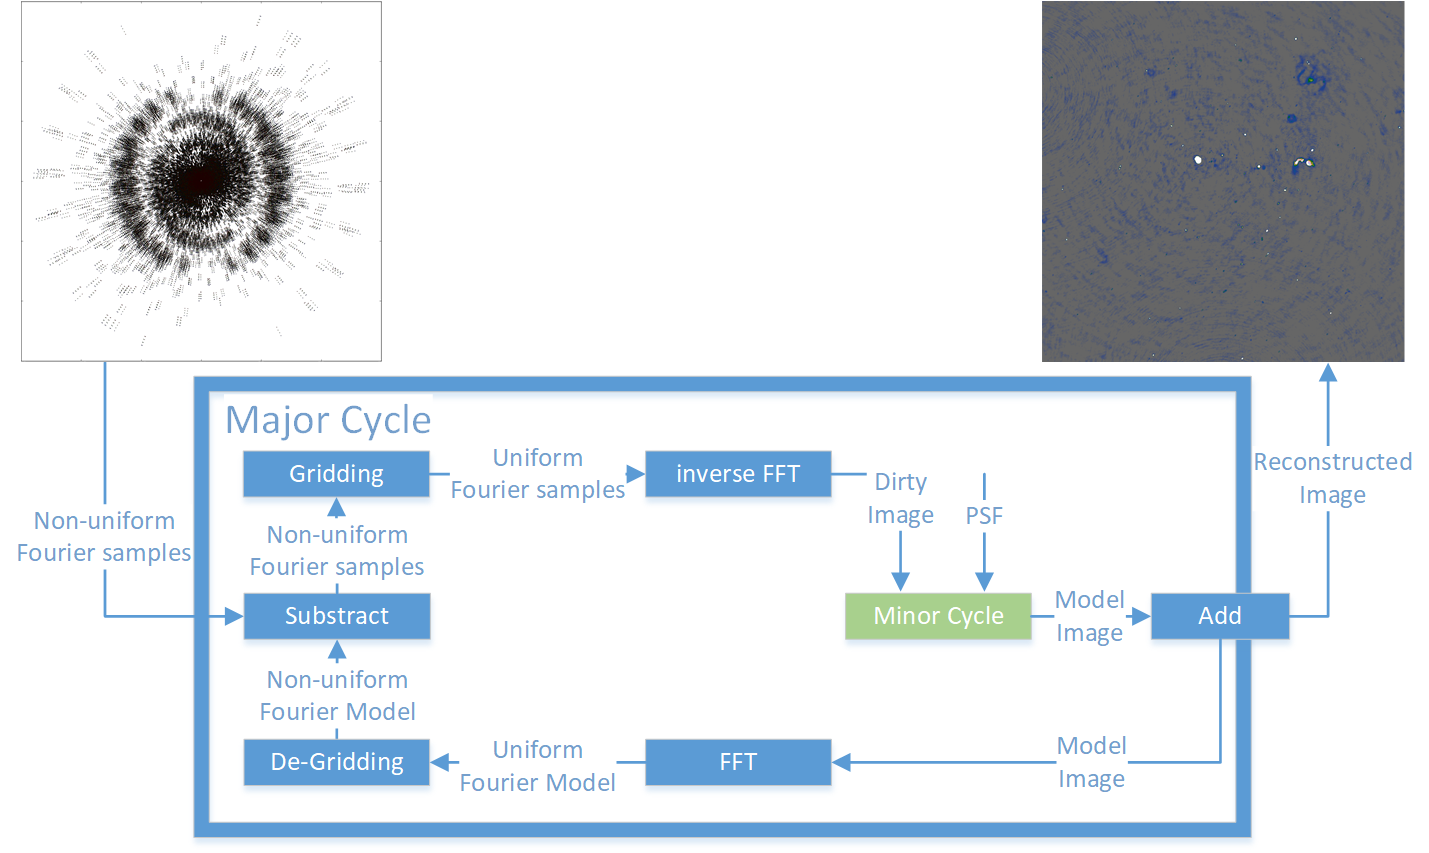
\includegraphics[width=0.90\linewidth]{./chapters/02.hypo/Major-Minor3.png}
	\caption{The Major/Minor Cycle Architecture}
	\label{intro:major:fig}
\end{figure}

The first half of the major cycle approximates the dirty image ($I_{dirty} \approx F^{-1}V$) for the minor cycle, while the second half takes the deconvolved image, called the "model" image in the major/minor cycle architecture, and transforms it back to the original visibility space ($V_{model} \approx Fx$). The next major cycle then uses the residual visibilities ($V_{res} = V - V_{model}$) and repeats the process.

At first glance, it may not be clear why several major cycles are even necessary. It is precisely this cycle that allows us to introduce approximations in the minor cycle. We will go into more detail about the approximations in section \ref{intro:major:approximations} and why they are important for radio interferometers.
This section dives deeper into the core operation of the major cycle, the gridding. 




\subsubsection{Approximations under the major cycle} \label{intro:major:approximations}
Looking at the deconvolution problem \eqref{intro:major:reformulation:deconv} in isolation , we find a few hidden difficulties with the $PSF$.

 For one, it spans the whole image and it is not constant over all pixels. DDE's like the $w$-term change the $PSF$ for each pixel. Solving the deconvolution problem would require us to estimate the $PSF$ for each pixel, which quickly becomes too expensive for larger images\footnote{Calculating the $PSF$ for a pixel requires a gridding and an iFFT step, or half a major cycle. We need around two to ten major cycles for an accurate reconstruction. Estimating a $PSF$ for each pixel is not viable.}. With the major cycle however, we can use an approximation of the true $PSF$. The error we introduce by approximating the $PSF$ will get removed over several major cycles. 

Typically, the minor cycle uses a constant $PSF$ and cuts parts of it off, only using the most significant center. An example is shown in figure \ref{intro:major:dynamic:psf} and \ref{intro:major:dynamic:psfCut}. The figure \ref{intro:major:dynamic:psf} shows the $PSF$ for the center pixel. It is approximately Gaussian shape in the center, but affects pixels over the whole image. Figure \ref{intro:major:dynamic:psfCut} shows the window which was used for deconvolution. It is half the size of the original $PSF$, and the minor cycle ignores all effects of the $PSF$ that are further away. 


he final reconstructed image is the sum of the model images over several major cycles. But this "backwards pass" is what allows us to: Reduce the error from interpolation and use a constant plus cropped $PSF$.

Interpolation error.

\begin{figure}[h]
	\centering
	\begin{subfigure}[b]{0.4\linewidth}
		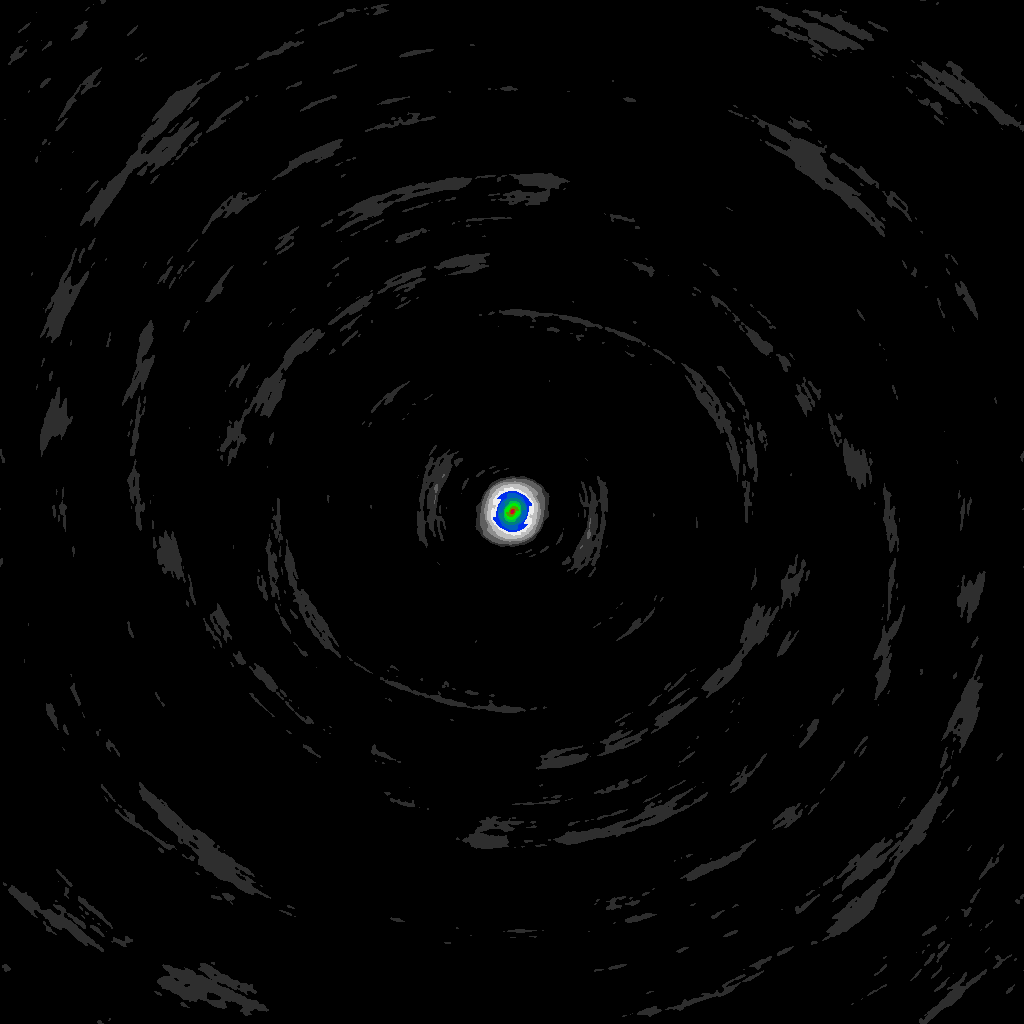
\includegraphics[width=\linewidth]{./chapters/01.intro/mk2/psf.png}
		\caption{$PSF$ for the center pixel.}
		\label{intro:major:dynamic:psf}
	\end{subfigure}
	\begin{subfigure}[b]{0.4\linewidth}
	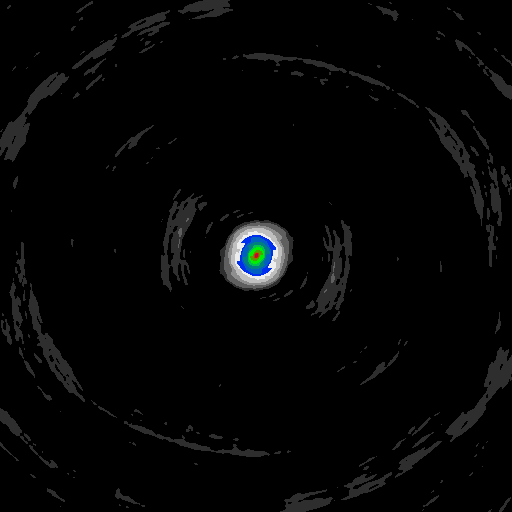
\includegraphics[width=\linewidth]{./chapters/01.intro/mk2/psfCut.png}
	\caption{$PSF$ window used for deconvolution.}
	\label{intro:major:dynamic:psfCut}
	\end{subfigure}

	
	\begin{subfigure}[b]{0.4\linewidth}
		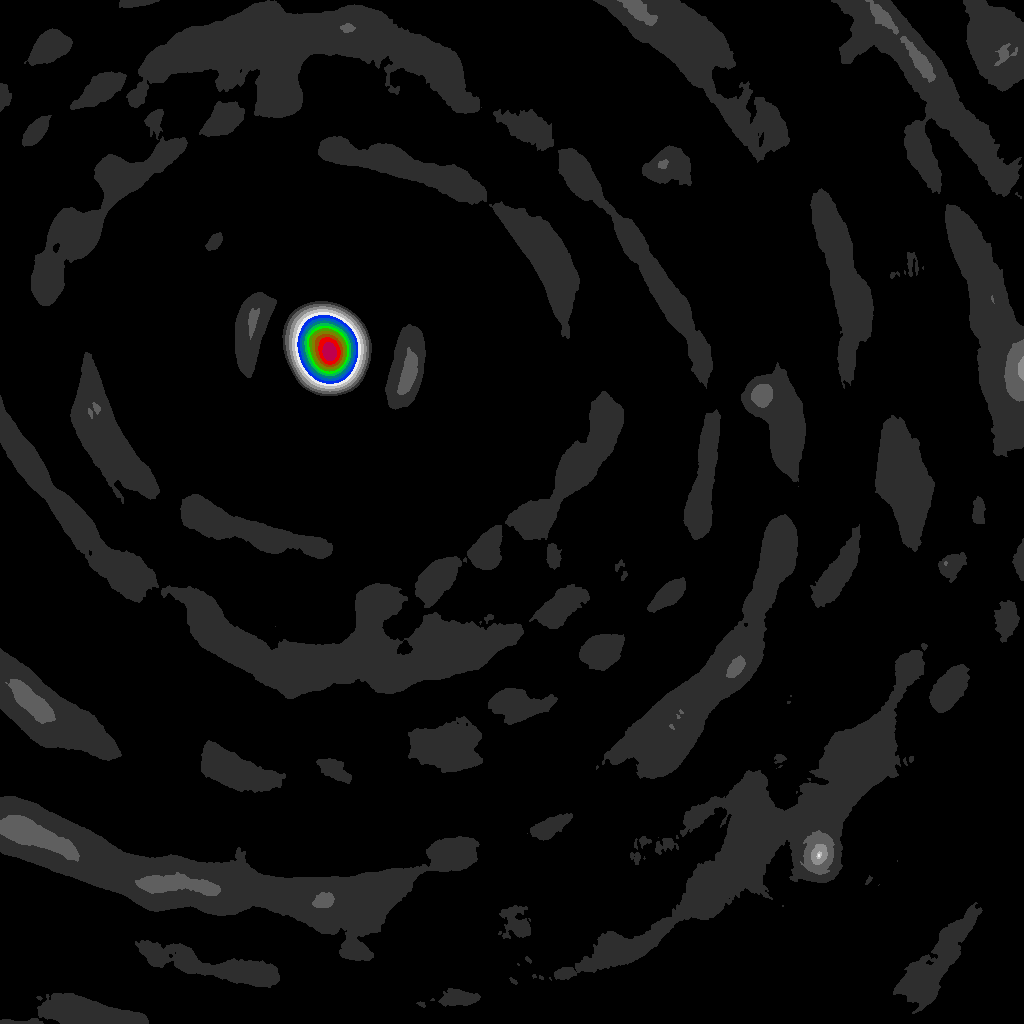
\includegraphics[width=\linewidth]{./chapters/01.intro/mk2/dirty.png}
		\caption{Dirty image.}
		\label{intro:major:dynamic:dirty}
	\end{subfigure}
	\begin{subfigure}[b]{0.4\linewidth}
		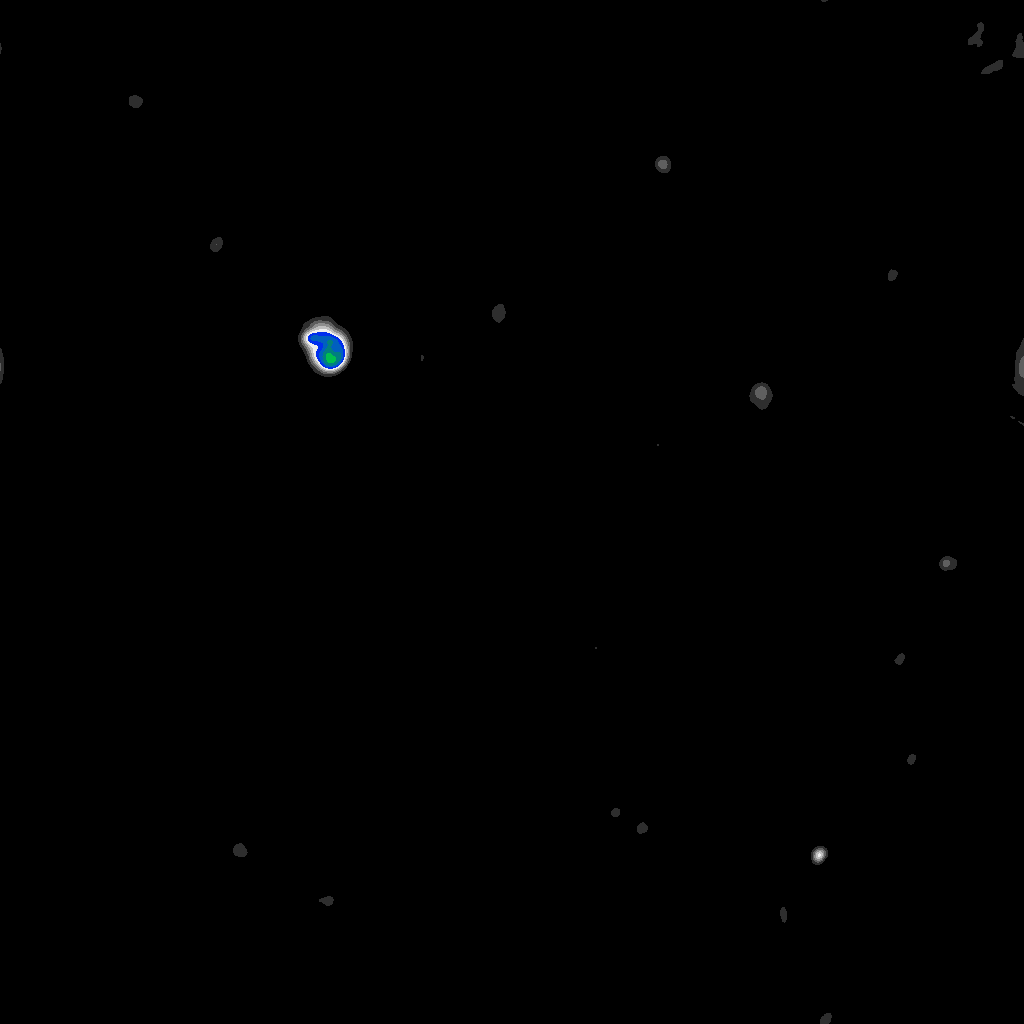
\includegraphics[width=\linewidth]{./chapters/01.intro/mk2/clean.png}
		\caption{Reconstructed image after 5 major cycles.}
		\label{intro:major:dynamic:tclean}
	\end{subfigure}
	
	\caption{Deconvolution problem for the MeerKAT radio interferometer with a strong extended emission and weaker point sources in the image.}
	\label{intro:major:dynamic}
\end{figure}


Figure \ref{intro:major:dynamic} shows a deconvolution problem for the MeerKAT radio interferometer. The $PSF$ for the center pixel is shown in figure \ref{intro:major:dynamic:psf}. The $PSF$ is approximately a gaussian at the center, with only

\eqref{intro:major:deconv}, $PSF$ is not constant. DDE like the $w$-term change the $PSF$ for each pixel. But estimating a $PSF$ is an expensive operation. In section \ref{dist} we show how the $PSF$ is estimated in practice. 
Several approximations. The minor cycle does not need to calculate the exact deconvolution, and the Gridding step is also just an approximation.

$PSF$ is not constant over the image. With the Major cycle, the minor cycle can approximate the deconvolution with a constant $PSF$. Estimating the $PSF$ for one location is as expensive as half a major cycle. It is common to use a single estimation for the whole problem

Assuming we know the reconstructed image, the major cycle then just improves the gridding accuracy, similar to how \cite{kunisnonequispaced}.
Several major cycles gives us free improved accuracy 



Alternatives to the major cycle


\subsubsection{Alternatives to the major/minor cycle architecture}





















Let us first look at the Major Cycle of figure \ref{intro:major} in more detail. We can separate


The first Major Cycle takes the calibrated, non-uniformly sampled Visibilities and interpolates them on a uniform Grid. This lets us use the inverse FFT in the next step, and the Cycle arrives at the Dirty Image. At this point, the Minor Cycle takes over and deduces the most likely observed image, the Model Image. After the Minor Cycle, the Major Cycle continues with the Model Image. It calculating the FFT and the De-Gridding on the model image, and finishes with non-uniformly sampled Model Visibilities. The second Major Cycle subtracts the Model from the calibrated Visibilities and repeats the process with the residuals.

In the real world, several Major Cycles, between 2-6 are needed to reconstruct an image.
At first glance, it is not clear why we cannot just use a single major cycle. The Minor Cycle minimizes the objective \eqref{intro:linear:repr:deconv}, it seems all we need is the $PSF$ and the Dirty Image from the first Major Cycle. The problem is that the $PSF$ of Radio Interferometers is not constant over the image. DDEs like the $w$-correction affect the $PSF$. In this architecture, we only approximate the deconvolution in the Minor Cycle. 

How many Minor Cycles, Major Cycles. We can use a fast approximation in the Minor Cycle. Minor Cycles are computationally cheap compared to the Major Cycle. For maximum speed, we would only want a single Major Cycle. But for the best reconstruction quality, we want as many as possible.

\subsubsection{Minor Cycle: CLEAN Deconvolutions}

The Minor Cycle was conceived with CLEAN in mind.
CLEAN is state of the art algorithm

Contains two classes of objects: Point sources, which are essentially stars, and extended emissions, which span over several pixels.


Find the fainter sources in later iterations
Because we can only estimate the psf.






